\documentclass[11pt,a4paper]{article}
\usepackage[a4paper,margin=1in]{geometry}
\usepackage{microtype}
\usepackage{amsmath,amssymb}
\usepackage{graphicx}
\usepackage{booktabs}
\usepackage{tabularx}
\usepackage{array}
\usepackage{listings}
\usepackage[font=small,labelfont=bf]{caption}
\usepackage{xurl}
\usepackage[hidelinks]{hyperref}
\hypersetup{pdftitle={Fair temporal model selection for Victorian rental medians},
            pdfauthor={Kelvin Valani}}
\lstset{basicstyle=\small\ttfamily, breaklines=true, columns=fullflexible,
        keepspaces=true, frame=single, framerule=0.2pt, xleftmargin=1em}
\setlength{\emergencystretch}{3em}
\title{Fair temporal model selection for Victorian rental medians}
\author{Kelvin Valani \\ \normalsize\href{https://github.com/kelvinvalani/vic-rent-ml}{\texttt{github.com/kelvinvalani/vic{-}rent{-}ml}}}
\date{\small Units: Australian dollars per week throughout \textperiodcentered{} Data: Homes Victoria Rental Report (RTBA bond lodgements), 2001 Q1 -- 2025 Q3}
\begin{document}
\maketitle

\begin{abstract}
We compare 24 learned forecasting configurations and two persistence baselines for Victorian suburb-group moving-annual median rents. Every candidate is scored under one recursive temporal protocol: expanding-window origins, eight-quarter forecasts that feed their own predictions back into lag features, and a single pre-registered objective. No family is preferred and no tree-over-linear hurdle is applied.

Huber regression on quarterly changes with postcode categories wins with equal-horizon validation MAE \textbf{23.80}, against \textbf{25.94} for the best tested XGBoost configuration and \textbf{25.98} for last-quarter persistence. The frozen winner is then audited once on 2025 Q1--Q3: MAE \textbf{14.87} versus \textbf{16.85} for persistence, an \textbf{11.74\%} reduction. A suburb-group cluster bootstrap puts the audit gap at \textbf{1.98} (95\% interval \textbf{1.45 -- 2.49}) AUD/week, so the ranking is stable to resampling whole suburb groups --- while remaining a statement about this panel, not a guarantee for the next regime.

The same estimator and features score \textbf{7.23} MAE under a shuffled 80/20 split and \textbf{12.04} under a one-step temporal split. The protocol, not the algorithm, drives most of the apparent accuracy in this problem class; we report the \textbf{23.80} figure because it is the only one that matches what the shipped artifact actually does.

These results concern aggregate rent medians, not individual property valuations, and do not establish that linear models generally outperform gradient boosting.
\end{abstract}

\section{Initial thinking}

The project began with a specific suspicion rather than a model wish-list. Rental dashboards routinely quote \(R^2 > 0.99\) on suburb rent data. That number is almost always an artifact: last quarter's median explains nearly all of this quarter's median, so any model that is shown the true previous value looks excellent. The starting question was therefore not \emph{which algorithm is best?} but \emph{what is the smallest honest number this problem admits, and does any learned model beat doing nothing?}

Four hypotheses were written down before the bake-off was run.

\begin{center}
\small
\begin{tabularx}{\linewidth}{@{}l>{\raggedright\arraybackslash}X>{\raggedright\arraybackslash}X@{}}
\toprule
\# & Starting hypothesis & Outcome \\
\midrule
H1 & Persistence will be a hard baseline, because the target is a smoothed moving-annual median. & \textbf{Supported.} Persistence (25.98) still beats 6 of the 24 learned configurations, including four boosting variants. \\
H2 & Gradient boosting will win, as it usually does on tabular panels. & \textbf{Not supported here.} The best XGBoost variant scores 25.94, behind all twelve linear and robust-linear configurations. \\
H3 & Level-targeted trees will clip during a boom, because a tree cannot extrapolate beyond its training leaves. & \textbf{Supported}, and pre-empted by modelling the change rather than the level. \\
H4 & Most of the measured accuracy will come from the evaluation protocol, not the estimator. & \textbf{Strongly supported} (Section 7.2): the same model spans 7.23 $\rightarrow$ 23.80 MAE across three protocols. \\
\bottomrule
\end{tabularx}
\end{center}

H2 failing is the interesting result, and it is reported as an outcome of \emph{this} specified grid on \emph{this} target --- not as a general claim about boosting. H4 is why the paper spends more space on the protocol than on the estimator.

\section{Target and source data}

Homes Victoria publishes the Rental Report from Residential Tenancies Bond Authority bond records. The target is the \textbf{moving-annual median weekly rent}, indexed by suburb group, dwelling type and bedroom count. Consecutive quarters describe overlapping annual windows. That smooths the series, induces strong serial dependence, and is precisely why recent-rent baselines must be taken seriously.

This run uses the historical transformed CSV bundled in \path{data/}. A fresh official workbook download is a different experiment; the bundled extraction has not been reconciled cell-by-cell against the current published workbook. This is a reproducible re-analysis of the repository data, not a claim to use the newest published file.

After requiring observed rents and exact calendar lag-1 and lag-4 values, the panel contains \textbf{82,025 rows}, \textbf{862 dwelling series} and \textbf{146 suburb groups}, spanning \textbf{2001 Q1 -- 2025 Q3}, with \textbf{142 observed representative postcodes}. The source's \texttt{CBD{-}St Kilda Rd} group has \textbf{297 rows without a postcode}; these keep an explicit missing category and remain addressable by group name. Bedroom categories 1--4 are supported; unsupported combinations are refused rather than assigned invented rents.

Lag construction joins series by exact quarter offsets --- a gap is never treated as one quarter merely because two rows are adjacent. Duplicate series-quarter keys, nonpositive rents and nonfinite required values are rejected. Scoring uses series observed at each origin whose future outcome exists; suppressed, missing or newly appearing series simply do not contribute. All errors carry equal row weight within a horizon: lease-count weighting answers a different, transaction-weighted question.

\section{Formal setup}

\subsection{Notation}

Let \(s\) index a series (suburb group $\times$ dwelling type $\times$ bedrooms) and \(t\) a quarter, encoded as \(t = 4\,\text{year} + \text{quarter}\). Write \(y_{s,t}\) for the observed moving-annual median weekly rent and \(x_{s,t}\) for the feature vector available at the \emph{end} of quarter \(t-1\):

\[
x_{s,t} = \big(\text{quarter}(t),\ \text{year}(t),\ \text{bedrooms}_s,\ y_{s,t-1},\ y_{s,t-4},\ \text{dwelling}_s,\ [\,\text{postcode}_s\,]\big),
\]

where the bracketed postcode term is present only in the \texttt{location} feature variant.

\subsection{Delta-innovation target}

Learned candidates predict the quarterly change rather than the level:

\[
\Delta_{s,t} = y_{s,t} - y_{s,t-1}, \qquad
\hat{y}_{s,t} = y_{s,t-1} + \hat{f}\!\left(x_{s,t}\right),
\]

so last-quarter persistence is the \emph{nested} model \(\hat f \equiv 0\), and every learned candidate is measured against the question ``can you improve on predicting no change?''.

\subsection{Recursive forecasting}

At forecast origin \(T\), horizons \(h = 1,\dots,H\) (with \(H = 8\)) are produced by feeding predictions back into the lag state:

\[
\hat{y}_{s,T+h} = \hat{y}_{s,T+h-1} + \hat{f}\!\left(\hat{x}_{s,T+h}\right),
\qquad \hat{y}_{s,T} \equiv y_{s,T},
\]

where \(\hat x_{s,T+h}\) uses \(\hat y_{s,T+h-1}\) as lag-1 and \(\hat y_{s,T+h-4}\) as lag-4 (falling back to \(y_{s,T}\) when an exact older lag is missing). No realised rent after \(T\) enters any feature. This is exactly the computation the shipped artifact performs, which is the point: the evaluation and the product run the same code path.

\subsection{Scoring}

With \(\mathcal{P}_h\) the set of forecast/outcome pairs at horizon \(h\):

\[
\mathrm{MAE}_h = \frac{1}{|\mathcal{P}_h|}\sum_{(s,t)\in\mathcal{P}_h}\left|\hat{y}_{s,t}-y_{s,t}\right|,
\qquad
\mathrm{RMSE}_h = \sqrt{\frac{1}{|\mathcal{P}_h|}\sum_{(s,t)\in\mathcal{P}_h}\left(\hat{y}_{s,t}-y_{s,t}\right)^{2}} .
\]

The selection score is the \textbf{equal-horizon mean}

\[
\overline{\mathrm{MAE}} = \frac{1}{H}\sum_{h=1}^{H}\mathrm{MAE}_h ,
\qquad
\overline{\mathrm{RMSE}} = \frac{1}{H}\sum_{h=1}^{H}\mathrm{RMSE}_h ,
\]

\emph{not} a pooled average over all pairs and \emph{not} the square root of pooled MSE. Pooling would let horizon 1 dominate simply because more of its outcomes are observable, quietly rewarding models that are good at the easy horizon. Ties in \(\overline{\mathrm{MAE}}\) go to \(\overline{\mathrm{RMSE}}\), then to the candidate identifier, so selection is deterministic.

\subsection{Uncertainty bands}

After the winner is frozen, each horizon's band half-width is the 80th percentile of absolute calibration-window error:

\[
w_h = Q_{0.80}\Big(\big\{\,|\hat{y}_{s,t}-y_{s,t}| : (s,t)\in\mathcal{C}_h\,\big\}\Big),
\qquad
\text{band}_h = \left[\hat{y}_{s,T+h}-w_h,\ \hat{y}_{s,T+h}+w_h\right],
\]

with \(\mathcal{C}_h\) the 2024 calibration pairs. These are empirical, symmetric and purely historical --- not a parametric predictive distribution, and not a claim about the spread of individual property rents.

\section{Design decisions and what each one costs}

Every choice below was made \emph{before} the audit window was touched. The right-hand column is the price paid for it, which is the part usually omitted.

\begin{center}
\small
\begin{tabularx}{\linewidth}{@{}>{\raggedright\arraybackslash}X>{\raggedright\arraybackslash}X>{\raggedright\arraybackslash}X>{\raggedright\arraybackslash}X@{}}
\toprule
Decision & Alternative rejected & Why & What it costs \\
\midrule
Predict \(\Delta\), anchor on \(y_{t-1}\) & Predict the level directly & Nominal rents trend; tree ensembles cannot emit a level above their highest training leaf and clip after a boom & Errors accumulate along the recursion; a biased \(\hat f\) drifts \\
Recursive eight-quarter scoring & One-step-ahead scoring & Production never has the realised lag-1 for horizon 5 & Roughly halves the headline accuracy (Section 7.2) \\
Expanding-window origins & Random 80/20 split & Overlapping moving-annual windows put the same information on both sides of a shuffle & Far fewer scored pairs; the pipeline refuses a panel that ends at the test origin \\
Equal-horizon mean & Pooled mean over all pairs & Stops horizon 1 dominating the ranking & Later, noisier horizons have more influence on selection \\
Two persistence baselines eligible to win & Learned-model-only shortlist & If nothing beats ``no change'', that is the finding & Risks shipping a baseline --- accepted \\
Exclude \texttt{lease\_count} & Use it, or impute a dummy at serving & Future lease counts do not exist; training on them is train/serve skew & Loses a genuinely informative historical signal \\
Exclude macro / amenity features & Add RBA, CPI, amenity snapshots & An eight-quarter forecast would need an invented exogenous path; amenity snapshots are not vintage-safe & No policy-scenario capability \\
Postcode as a category (\texttt{location} variant) & Suburb-group one-hot, or embeddings & Coarse geography, few parameters, degrades gracefully on unseen values & Only a 0.06 AUD/week gain --- kept for interpretability, not demonstrated skill \\
Huber loss \((\epsilon = 1.35)\) & Squared loss & Quarterly changes have heavy tails (regime shifts, small-sample groups) & Slightly biased under genuinely Gaussian noise \\
Freeze the winner before the audit & Re-rank all candidates on 2025 & Prevents the audit from becoming a second selection round & The audit says nothing about non-winning candidates \\
Refit the \emph{exact} selected pipeline on all data & Retrain a ``similar'' model for production & Eliminates selection/deployment mismatch & Refit coefficients are not the ones validated \\
\bottomrule
\end{tabularx}
\end{center}

\section{Candidates}

Ordinary least squares, Ridge (\(\alpha = 10\)), Lasso (\(\alpha = 0.1\)), Elastic Net (\(\alpha = 0.1\), \texttt{l1\_ratio} 0.5), Huber (\(\epsilon = 1.35\), 2000 iterations), Bayesian Ridge, histogram gradient boosting (200 iterations, 15 leaves, L2 = 10), random forest and Extra Trees (150 trees, depth 12, min leaf 10), gradient boosting (200 trees, depth 3, learning rate 0.05), and XGBoost at depths 3 and 6 (300 trees, learning rate 0.05, min child weight 10, L2 = 10, row/column subsample 0.8, \texttt{hist}). Each learned estimator is run under both feature variants; randomized estimators use seed 42. Full settings are in \path{docs/results/candidate_parameters.json}.

This is a finite specified grid, not exhaustive hyperparameter search --- a real limitation for the tree families, which are more tuning-sensitive than the linear ones. Numeric imputation and scaling and categorical one-hot encoding are fitted \textbf{inside} each fold.

\section{Temporal protocol}

\begin{figure}[!htbp]
\centering
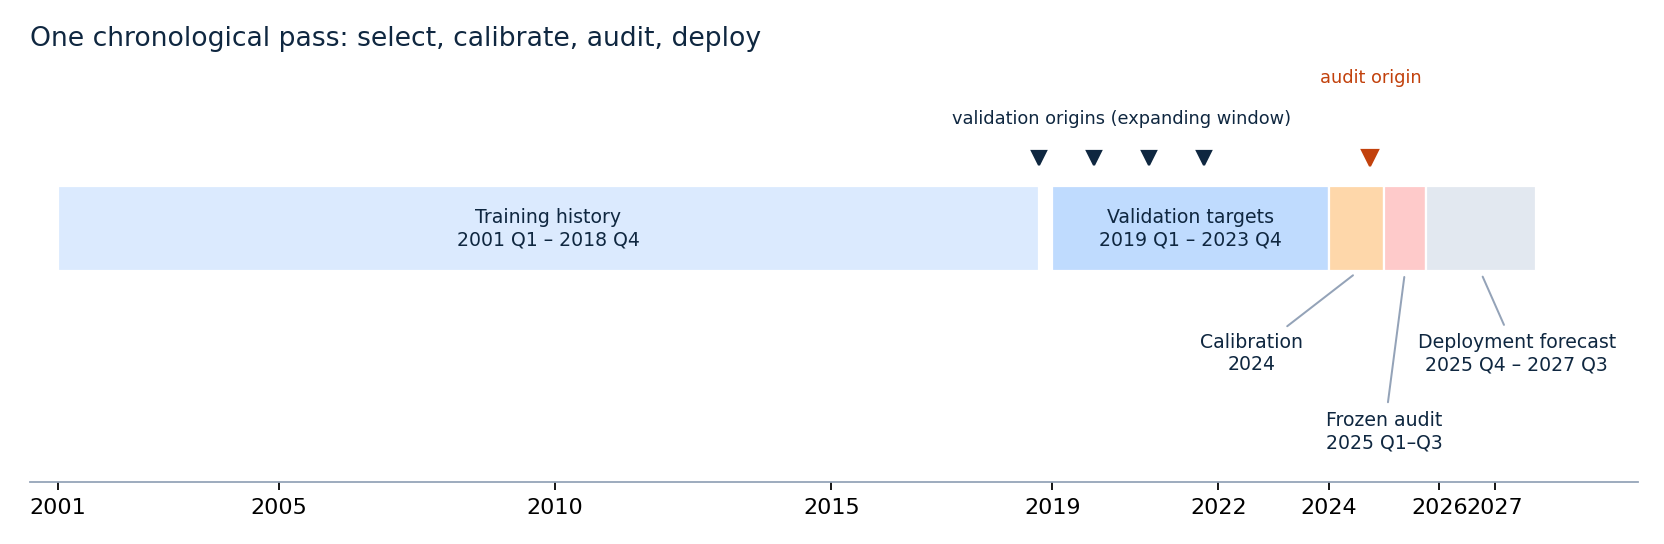
\includegraphics[width=\linewidth]{figures/evaluation_timeline.png}
\caption{One chronological pass: expanding validation origins select the candidate, 2024 calibrates the bands, a single frozen audit at the 2024 Q4 origin measures 2025 Q1--Q3, and the refit ships forecasts to 2027 Q3.}
\end{figure}

\begin{center}
\small
\begin{tabularx}{\linewidth}{@{}l>{\raggedright\arraybackslash}X>{\raggedright\arraybackslash}X>{\raggedright\arraybackslash}X@{}}
\toprule
Stage & Origins & Scored targets & Purpose \\
\midrule
Validation & Expanding history ending Q4 of 2018, 2019, 2020, 2021 & Next 8 quarters per origin, no later than 2023 Q4 & Choose the candidate \\
Calibration & Expanding origins 2022 Q1 -- 2024 Q3 & Targets in 2024 only, horizons 1--8 & Fit band half-widths \\
Frozen audit & One origin, 2024 Q4 & Available 2025 Q1--Q3 outcomes & Audit winner vs baselines \\
Deployment refit & All labelled data through 2025 Q3 & Forecasts to 2027 Q3 & Serve the selected pipeline \\
\bottomrule
\end{tabularx}
\end{center}

All 26 candidates see the same \textbf{26,651} validation forecast/outcome pairs, and no convergence warnings were recorded. Test metrics never enter the ranking. Only three test horizons are observable, so this experiment provides \textbf{no final-test result for horizons 4--8} --- the bands at those horizons are calibrated but unaudited.

The chronological partition blocks direct future-target leakage. It is \emph{not} a full vintage simulation: quarter-end reference dates are used as availability dates, so publication delay and retrospective revision remain unmodelled.

\section{Results}

\subsection{Validation selection}

\begin{figure}[!htbp]
\centering
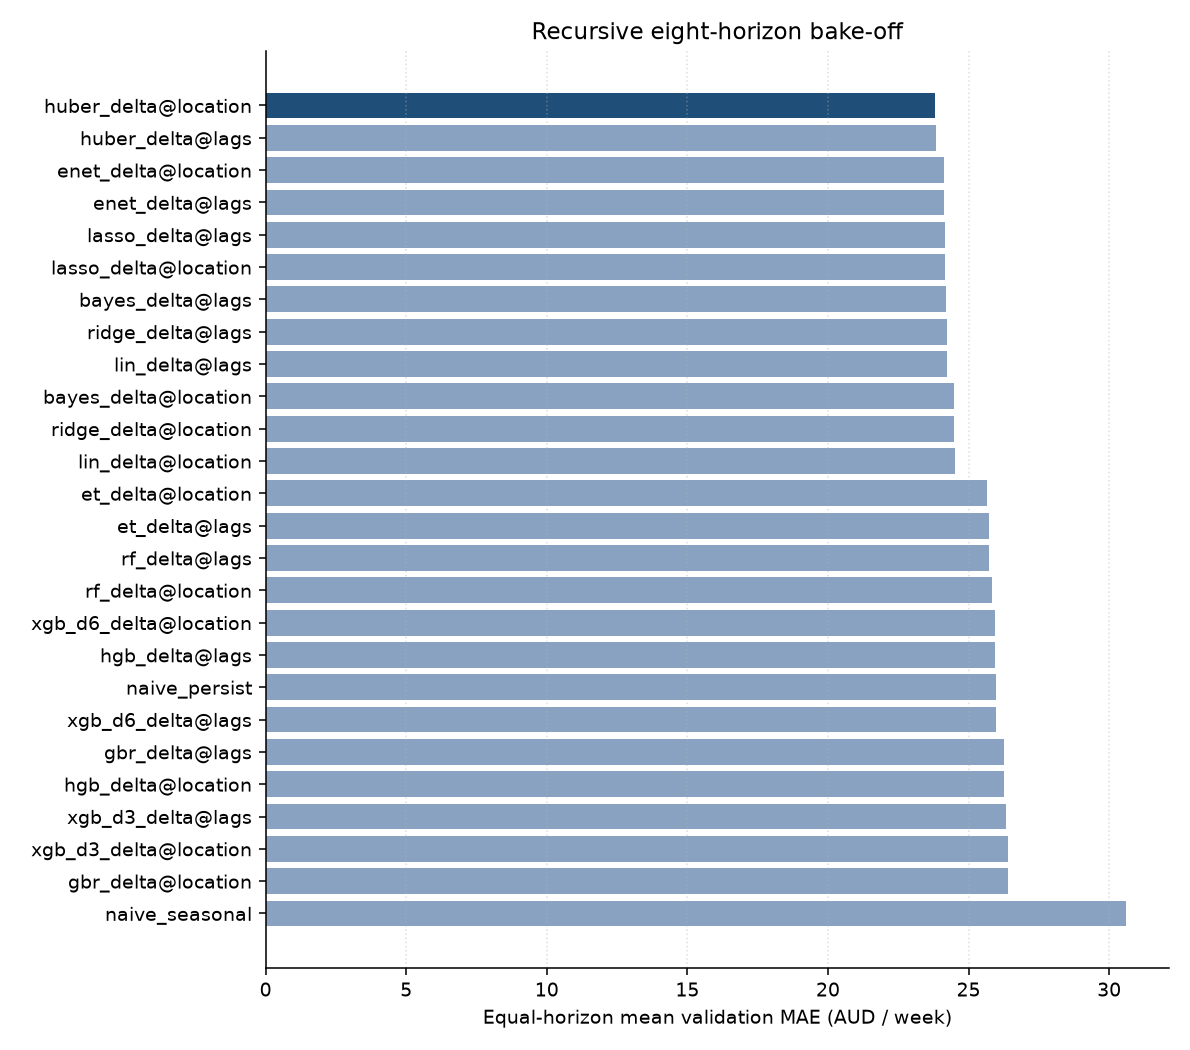
\includegraphics[width=\linewidth]{figures/validation_mae.png}
\caption{Equal-horizon mean validation MAE for all 26 candidates. Huber with postcode categories is lowest; the dashed line is last-quarter persistence, which still beats six learned configurations.}
\end{figure}

Best feature variant per family (the full 26-row ranking is in \path{docs/results/bakeoff_metrics.csv}):

\begin{center}
\small
\begin{tabularx}{\linewidth}{@{}>{\raggedright\arraybackslash}Xl>{\raggedright\arraybackslash}X>{\raggedright\arraybackslash}X@{}}
\toprule
Candidate & Features & Validation MAE & Validation RMSE \\
\midrule
\textbf{Huber} & \textbf{location} & \textbf{23.80} & \textbf{37.22} \\
Elastic Net & lags / location tie & 24.14 & 37.45 \\
Lasso & lags / location tie & 24.17 & 37.40 \\
Bayesian Ridge & lags & 24.22 & 37.53 \\
Ridge & lags & 24.22 & 37.53 \\
Ordinary least squares & lags & 24.22 & 37.53 \\
Extra Trees & location & 25.65 & 39.82 \\
Random forest & lags & 25.74 & 40.35 \\
XGBoost, depth 6 & location & 25.94 & 40.85 \\
Histogram gradient boosting & lags & 25.94 & 40.68 \\
Last-quarter persistence & --- & 25.98 & 39.44 \\
Gradient boosting & lags & 26.25 & 40.00 \\
XGBoost, depth 3 & lags & 26.32 & 40.31 \\
Seasonal persistence & --- & 30.60 & 45.19 \\
\bottomrule
\end{tabularx}
\end{center}

Huber improves on persistence by \textbf{8.40\%}. Adding postcode moves Huber only from \textbf{23.857} to \textbf{23.799} --- a descriptive difference of 0.06 AUD/week, not evidence of a reliable location effect. The rule nevertheless selects the lower score, exactly as it would have for a similarly small tree advantage.

\begin{figure}[!htbp]
\centering
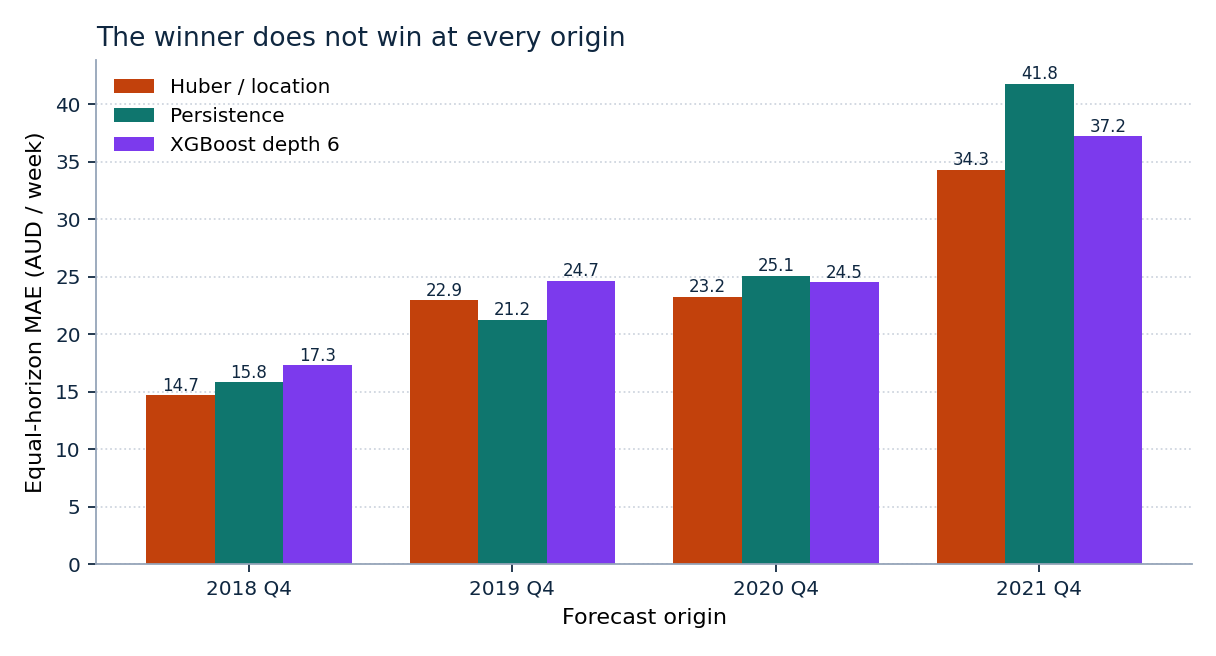
\includegraphics[width=\linewidth]{figures/origin_variation.png}
\caption{Per-origin MAE. The 2021 Q4 origin is the hardest window for every model, and persistence wins the 2019 Q4 origin outright.}
\end{figure}

\begin{center}
\small
\begin{tabularx}{\linewidth}{@{}l>{\raggedright\arraybackslash}X>{\raggedright\arraybackslash}X>{\raggedright\arraybackslash}X@{}}
\toprule
Origin & Huber/location MAE & Persistence MAE & XGBoost depth-6/location MAE \\
\midrule
2018 Q4 & 14.70 & 15.81 & 17.31 \\
2019 Q4 & 22.95 & \textbf{21.25} & 24.66 \\
2020 Q4 & 23.24 & 25.05 & 24.53 \\
2021 Q4 & 34.27 & 41.77 & 37.21 \\
\bottomrule
\end{tabularx}
\end{center}

The winner does not beat persistence at every origin. Strong persistence plus strong robust linear performance is consistent with a smooth target and heavy-tailed changes; Huber's reduced outlier sensitivity is a plausible explanation, not a causal finding.

\subsection{The protocol, not the model, sets the headline}

\begin{figure}[!htbp]
\centering
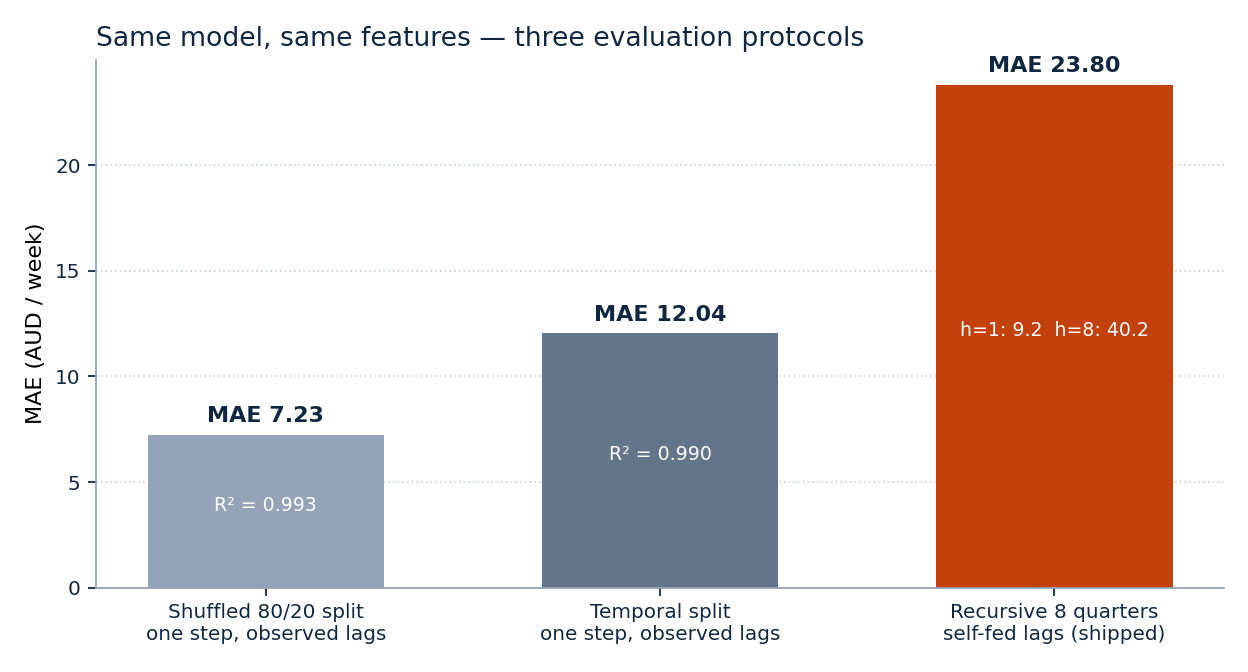
\includegraphics[width=\linewidth]{figures/protocol_illusions.png}
\caption{The same Huber/location estimator and features under three evaluation protocols. Only the right-hand bar corresponds to what the shipped model does.}
\end{figure}

Holding the estimator and features fixed and changing only the evaluation protocol (\path{docs/build/evaluation_illusions.py}):

\begin{center}
\small
\begin{tabularx}{\linewidth}{@{}>{\raggedright\arraybackslash}Xrrr@{}}
\toprule
Protocol & MAE & Level \(R^2\) & Pairs \\
\midrule
Shuffled 80/20 split, one step, observed lags & 7.23 & 0.9934 & 15,239 \\
Temporal split, one step, observed lags & 12.04 & 0.9895 & 6,708 \\
\textbf{Recursive 8 quarters, self-fed lags (shipped)} & \textbf{23.80} & --- & 26,651 \\
\bottomrule
\end{tabularx}
\end{center}

A shuffled split lets overlapping moving-annual windows and neighbouring quarters of the same series appear on both sides of the partition; one-step scoring hands the model an observed lag it will never have at horizon 5. Either choice would have made this project look three times better and would have been wrong. Within the recursive protocol, error grows from \textbf{9.16} at \(h=1\) to \textbf{40.24} at \(h=8\) --- an honest description of how far ahead this target is actually predictable.

\subsection{Frozen-winner audit}

\begin{center}
\small
\begin{tabular}{@{}lrrr@{}}
\toprule
Model & Test MAE & Test RMSE & Pairs \\
\midrule
\textbf{Huber/location} & \textbf{14.87} & \textbf{28.19} & 2,472 \\
Last-quarter persistence & 16.85 & 29.51 & 2,472 \\
Seasonal persistence & 34.30 & 45.17 & 2,472 \\
\bottomrule
\end{tabular}
\end{center}

These are equal-horizon averages over the \textbf{three} observable test horizons, so they are not comparable with the eight-horizon validation average; the audit window is also simply calmer than 2021--22. The winner was frozen before this audit and no other candidate was re-ranked on it.

\begin{figure}[!htbp]
\centering
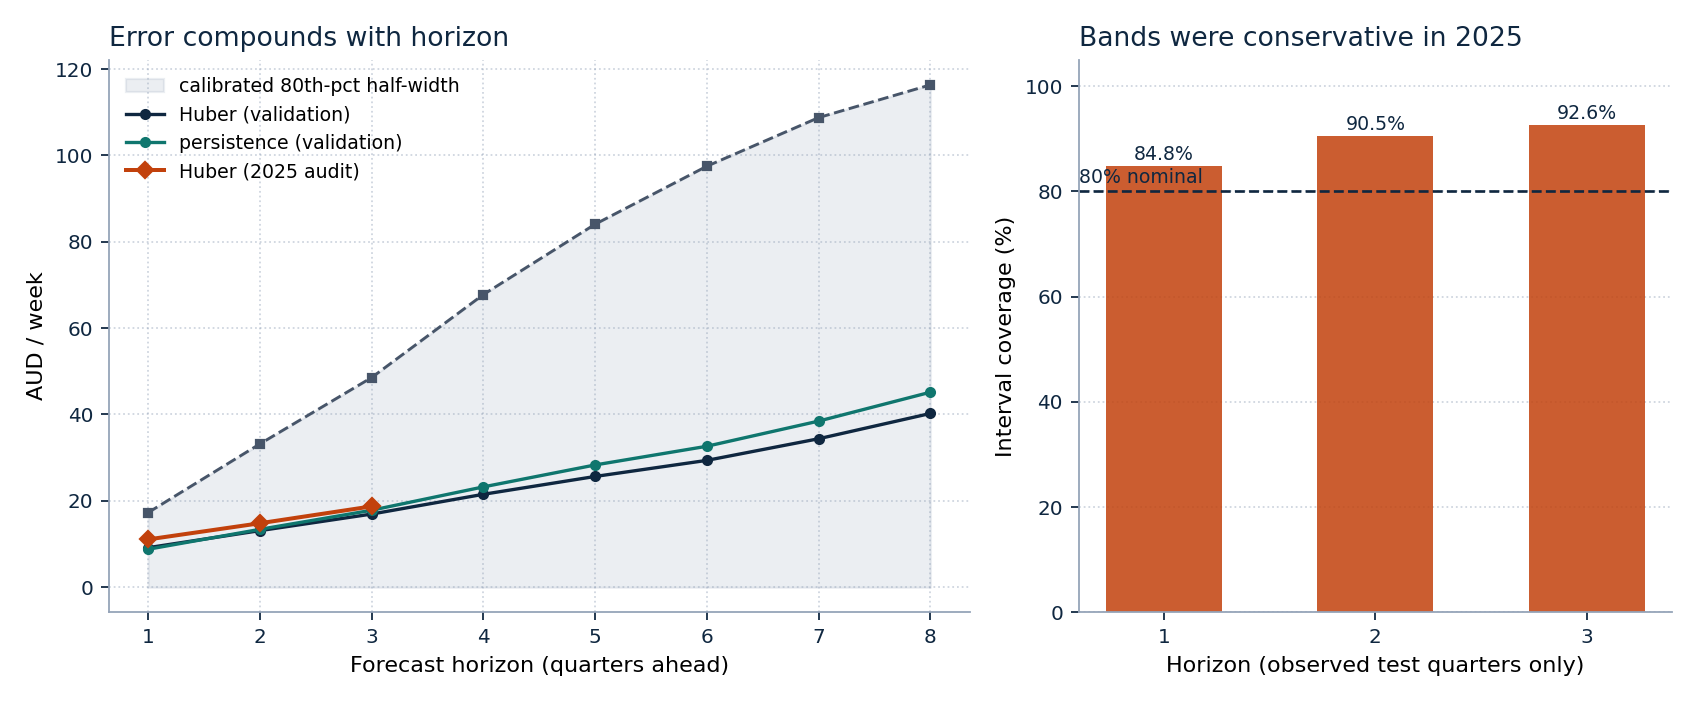
\includegraphics[width=\linewidth]{figures/horizon_errors.png}
\caption{Left: per-horizon validation MAE for Huber and persistence against the calibrated 80th-percentile half-width. Right: observed audit coverage at the only three horizons with outcomes.}
\end{figure}

\begin{center}
\small
\begin{tabularx}{\linewidth}{@{}lrr>{\raggedright\arraybackslash}X>{\raggedright\arraybackslash}X@{}}
\toprule
Horizon & Test pairs & MAE & Empirical half-width & Observed coverage \\
\midrule
1 quarter & 829 & 11.07 & 17.29 & 84.80\% \\
2 quarters & 822 & 14.82 & 33.19 & 90.51\% \\
3 quarters & 821 & 18.73 & 48.56 & 92.57\% \\
4 quarters & not observed & --- & 67.78 & --- \\
5 quarters & not observed & --- & 84.07 & --- \\
6 quarters & not observed & --- & 97.50 & --- \\
7 quarters & not observed & --- & 108.75 & --- \\
8 quarters & not observed & --- & 116.33 & --- \\
\bottomrule
\end{tabularx}
\end{center}

Coverage exceeds the nominal 80\% at every observed horizon, which says the 2024 calibration errors were conservative for this particular 2025 period --- not that coverage is guaranteed in the next regime.

\subsection{How much of the gap is sampling noise?}

Rows are not independent: 2,472 audit pairs come from 829 series inside only 146 suburb groups. Treating them as independent would overstate precision. We therefore resample \textbf{whole suburb groups} with replacement (2,000 draws, seed 42, \path{docs/build/analysis.py}), recomputing the equal-horizon MAE gap between the winner and persistence on each draw.

\begin{center}
\small
\begin{tabularx}{\linewidth}{@{}>{\raggedright\arraybackslash}Xrr>{\raggedright\arraybackslash}Xr>{\raggedright\arraybackslash}X>{\raggedright\arraybackslash}Xr@{}}
\toprule
Window & Pairs & Winner MAE & Persistence MAE & Gap & 95\% cluster-bootstrap interval & Draws favouring winner & Series won \\
\midrule
Validation (2019 Q1 -- 2023 Q4) & 26,651 & 23.80 & 25.98 & \textbf{2.18} & [1.60, 2.79] & 100\% & 64.6\% \\
Frozen audit (2025 Q1 -- Q3) & 2,472 & 14.87 & 16.85 & \textbf{1.98} & [1.45, 2.49] & 100\% & 63.2\% \\
\bottomrule
\end{tabularx}
\end{center}

The interval excludes zero in both windows and no bootstrap draw reverses the ranking, so the advantage is not an artifact of a few influential suburb groups. Two caveats keep this honest: the interval describes resampling variability of the \emph{measured} gap on this panel, not out-of-sample performance under a regime change; and the winner still loses on \textasciitilde{}36\% of individual series.

\subsection{Where the error actually lives}

\begin{figure}[!htbp]
\centering
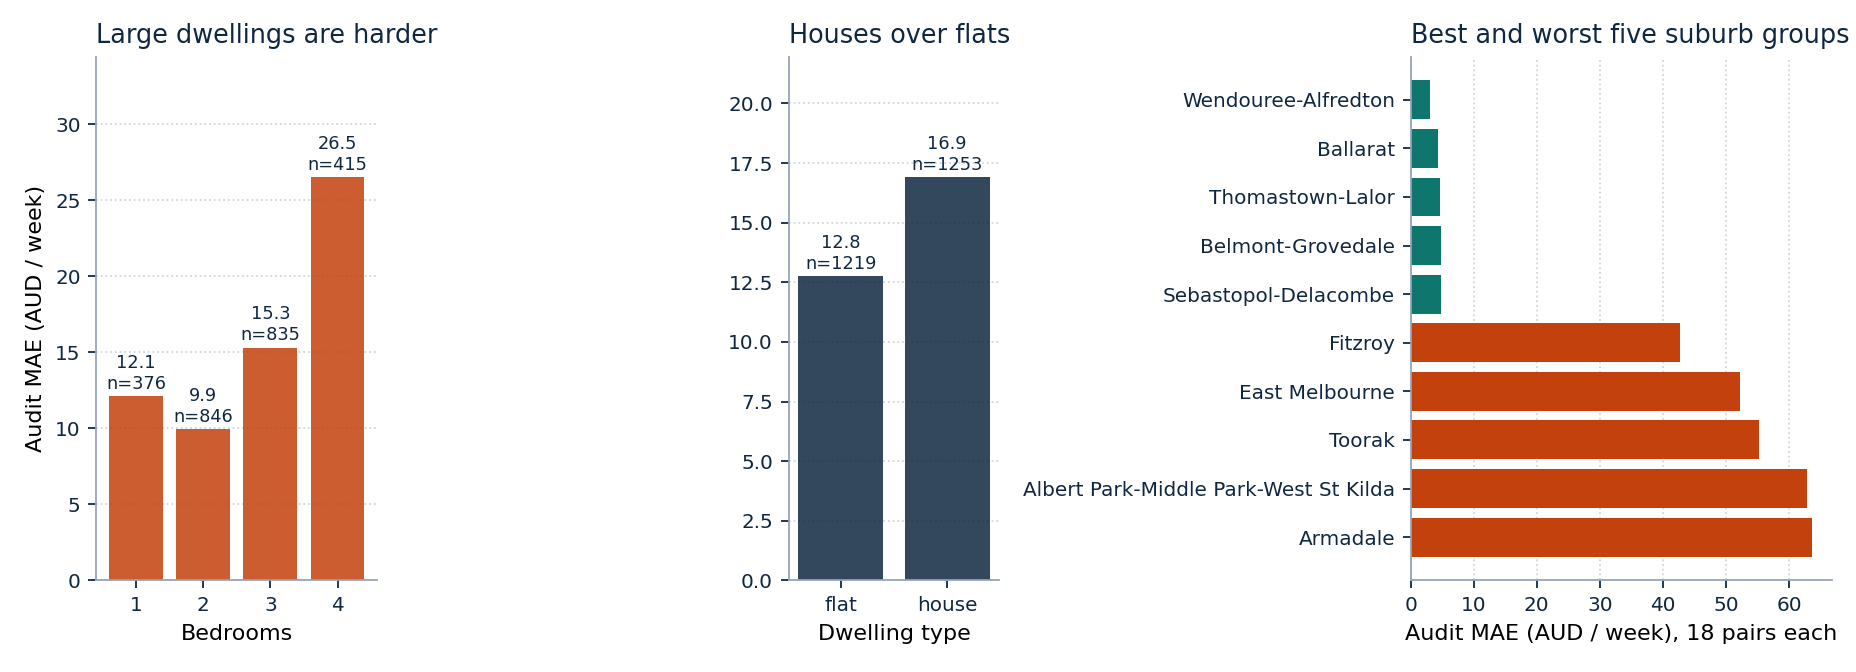
\includegraphics[width=\linewidth]{figures/slice_errors.png}
\caption{Audit MAE by bedrooms, by dwelling type, and for the five best and five worst suburb groups.}
\end{figure}

Pooled audit MAE is \textbf{12.77} for flats and \textbf{16.90} for houses, and rises from \textbf{9.94} for two-bedroom to \textbf{26.50} for four-bedroom dwellings --- thin, expensive, volatile slices are the hard ones. Armadale reaches MAE \textbf{63.64} on only 18 pairs; Albert Park--Middle Park--West St Kilda \textbf{62.87} and Toorak \textbf{55.31} on the same slice size. Average performance conceals substantial local error, and these per-group figures are too small to support significance claims of their own.

\subsection{What the shipped model actually forecasts}

\begin{figure}[!htbp]
\centering
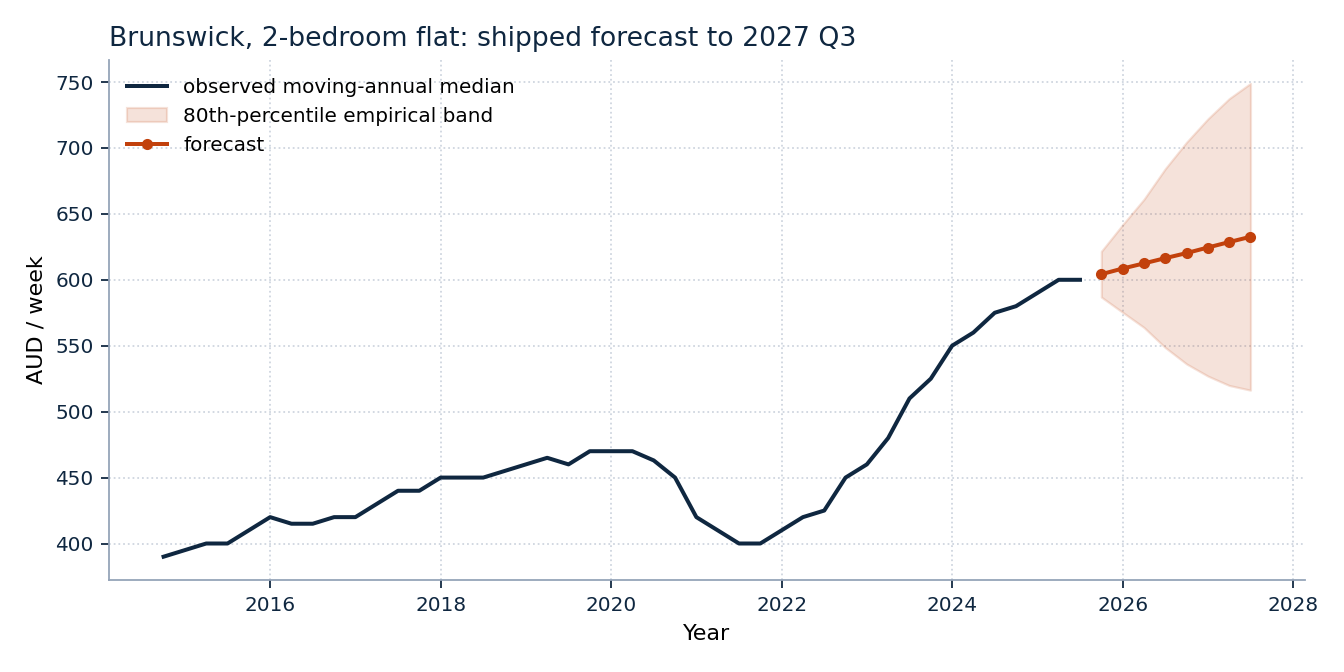
\includegraphics[width=\linewidth]{figures/forecast_example.png}
\caption{Brunswick two-bedroom flats: observed history, the deployment forecast to 2027 Q3, and the calibrated band widening from $\pm$17 to $\pm$116 AUD/week.}
\end{figure}

For Brunswick two-bedroom flats (anchor 600 AUD/week at 2025 Q3), the refit model forecasts 604 AUD/week for 2025 Q4 (band 587--622) and 633 for 2027 Q3 (band 516--749). The point path is close to a gentle linear rise; the honest content of the forecast is the band, which nearly quadruples in width over eight quarters. Full per-series forecasts are in \path{docs/results/deployment_forecasts.csv}.

\section{What this model does not do}

\begin{itemize}
\item It does \textbf{not} value individual properties. The bands describe the error of a \emph{group median}, and must never be read as the range containing 80\% of individual rents.
\item It does \textbf{not} establish that linear models beat gradient boosting in general --- only that in this grid, on this target, under this protocol, they did.
\item It does \textbf{not} explain \emph{why} rents move. There are no causal claims; postcode and bedroom effects are associations within a specific forecasting pipeline.
\item It has \textbf{no audited accuracy beyond three quarters ahead}. Horizons 4--8 ship with calibrated but unverified bands.
\item It assumes the measurement process is stable. A change in RTBA lodgement coverage, suppression rules or the moving-annual definition would break the lag relationships the model relies on, silently.
\item It carries no vintage realism: revisions and publication delays are not simulated.
\end{itemize}

\section{Open gaps and the next experiment}

\begin{enumerate}
\item \textbf{Vintage-correct data.} Reconstruct the as-published series with real availability dates, then re-run the protocol. This is the single biggest credibility gap.
\item \textbf{An independent eight-horizon audit.} Requires roughly five more quarters of outcomes; until then horizons 4--8 are unverified.
\item \textbf{A real tuning budget for the tree families}, using validation data only. The current grid is fixed and arguably under-serves boosting.
\item \textbf{Quantile or conformal intervals} instead of symmetric empirical half-widths, which cannot express asymmetric downside risk in falling markets.
\item \textbf{Hierarchical pooling} across suburb groups, targeted at the thin four-bedroom and high-price slices where error concentrates.
\item \textbf{Drift monitoring in production}: compare realised quarters against the shipped bands and alert when observed coverage departs from nominal.
\end{enumerate}

\section{Reproducibility}

\texttt{vic{-}rent{-}ml train} freezes the winner identifier, calibrates bands, audits the test window against persistence, and refits the exact selected pipeline on all labelled quarters. The schema-2 artifact stores the fitted estimator, origin history, precomputed recursive forecasts, residual widths, winner, evaluation plan, dependency versions and data digests. Saved-selection reuse (\texttt{{-}{-}reuse{-}selection}) fails if validation data, training source or evaluation settings change. Serving reads artifact history rather than fabricating amenity values or lease counts. Postcodes that map to more than one source group return an aggregated, flagged forecast; unsupported combinations fail instead of inventing a rent.

\begin{lstlisting}
python -m venv .venv && source .venv/bin/activate
pip install -r requirements-model.txt
pip install -e ".[dev]"
vic-rent-ml train --panel data/rent_panel.csv --out artifacts/production_clone.joblib --reuse-selection
python docs/build/analysis.py              # bootstrap intervals + deployment forecasts
python docs/build/evaluation_illusions.py  # protocol comparison
python docs/build/figures.py               # all figures in docs/figures/
python docs/build/explainer.py             # poster + explainer gif
python docs/build/paper.py                 # docs/vic-rent-ml-paper.{tex,pdf} (needs a TeX engine)
\end{lstlisting}

The published artifact run used Python \textbf{3.12.3}, NumPy \textbf{2.4.6}, pandas \textbf{3.0.6}, scikit-learn \textbf{1.9.1}, XGBoost \textbf{3.4.1}, joblib \textbf{1.6.0}; \texttt{manifest.json} records model SHA-256 \texttt{5839b40f1c04ae6646b178e66f21a5dc34742fb801459cb7c744afbe9afac56d}. The analyses in Sections 7.2 and 7.4 were re-run independently on Python 3.10.12 with NumPy 2.2.6, pandas 2.3.3, scikit-learn 1.7.2 and XGBoost 3.2.0, reproducing the published audit MAE of 14.871824 to seven significant figures (\path{docs/results/reproduction.json}). Only load trusted joblib artifacts with compatible dependencies.

\section{References and attribution}

\begin{enumerate}
\item Homes Victoria, \href{https://discover.data.vic.gov.au/dataset/rental-report-quarterly-moving-annual-rents-by-suburb}{Rental Report --- Quarterly: Moving Annual Rents by Suburb}. DataVic identifies the source licence as Creative Commons Attribution 4.0 International; retain Homes Victoria attribution when redistributing its data.
\item Hyndman and Athanasopoulos, \href{https://otexts.com/fpp3/tscv.html}{Forecasting: Principles and Practice --- Time series cross-validation}.
\item Huber (1964), Robust Estimation of a Location Parameter, \emph{Annals of Mathematical Statistics} 35(1), 73--101.
\item Efron (1979), Bootstrap Methods: Another Look at the Jackknife, \emph{Annals of Statistics} 7(1), 1--26; cluster variant per Cameron, Gelbach and Miller (2008).
\item scikit-learn, \href{https://scikit-learn.org/stable/modules/generated/sklearn.linear\_model.HuberRegressor.html}{HuberRegressor} and \href{https://scikit-learn.org/stable/common\_pitfalls.html}{Common pitfalls}.
\item Chen and Guestrin (2016), \href{https://doi.org/10.1145/2939672.2939785}{XGBoost: A Scalable Tree Boosting System}.
\end{enumerate}

\end{document}
